\chapter{Methods}

\section{Ahmad Syafrizal Huda / 1164062}
\subsection{Teori}
\begin{enumerate}
\item Random forest ialah sekumpulan classifier yang terdiri dari banyak pohon keputusan dan mengerjakan klasifikasi berdasarkan keluaran dari hasil klasifikasi setiap pohon keputusan anggota. Klasifikasi random forest dikerjakan melalui penggabungan pohon (tree) dengan melakukan training pada sampel data yang dimiliki. Contoh ilustrasi gambar random forest pada gambar \ref{h1}.
\begin{figure}[!htbp]
	\centerline{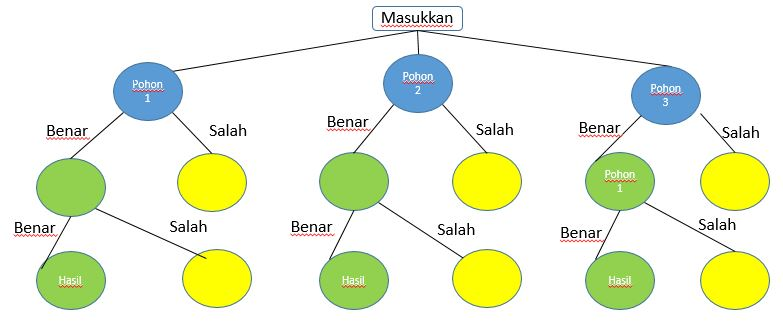
\includegraphics[width=1\textwidth]{figures/huda/chapter3/1.JPG}}
	\caption{Random Forest}
	\label{h1}
\end{figure}
\item Cara membaca dataset kasus dan makna setiap file dan isi field masing-masing file
\subitem Gunakan librari pandas yang sudah di install sebelumnya pada python untuk dapat membaca dataset dengan format text file.
\subitem  Selanjutnya buatlah variabel baru misalkan diberi nama dataset yang berisikan perintah untuk membaca file csv.
\begin{verbatim}
import pandas as data
dataset = data.read_csv("car.txt")
dataset.head()
\end{verbatim}
\subitem Pada perintah diatas yaitu memanggil library pandas untuk membaca dataset, membuat variabel dataset yang berisikan data.read\_csv untuk membaca dataset. Pada contoh ini menggunakan txt tapi tetap bisa membaca datasetnya, karena pada saat dijalankan librari pandas secara otomatis akan mengubah data dalam bentuk text file ke format csv. Hasilnya seperti pada gambar \ref{h2}.
\begin{figure}[!htbp]
	\centerline{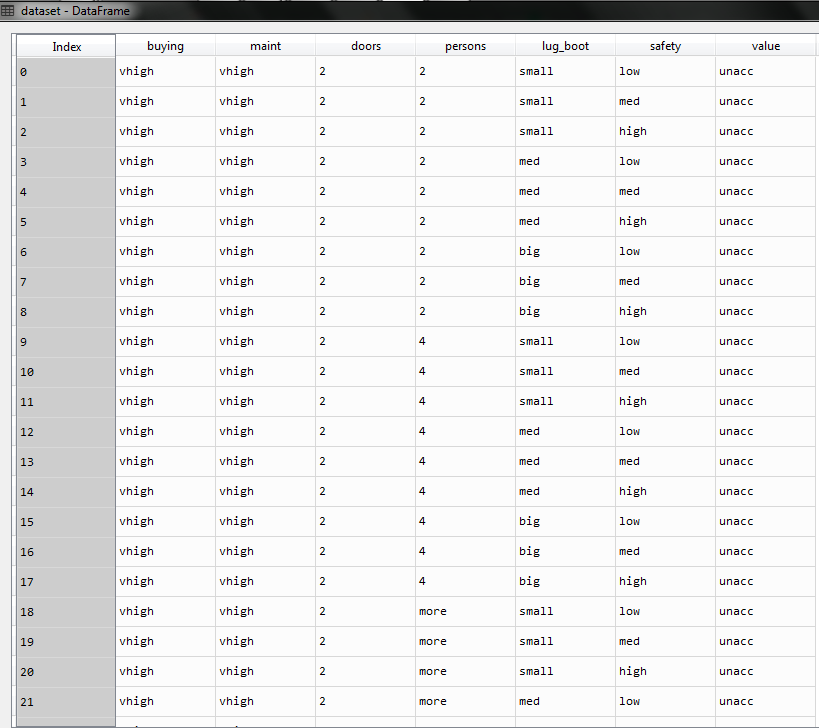
\includegraphics[width=1\textwidth]{figures/huda/chapter3/2.PNG}}
	\caption{Hasil Dataset}
	\label{h2}
\end{figure}
\subitem Penjelasan dari isi field pada hasil gambar \ref{h2} yaitu: Atribut Index merupakan atribut otomatis untuk penomoran data yang sudah ada, Atribut Buying merupakan harga beli dari mobil tersebut. dengan value : v high/Sangat mahal,high/mahal,med/Cukup, low/Murah, Atribut Maint merupakan harga perawatan dari mobil tersebut, dengan value sama seperti pada atribut Buying, Atribut Doors merupakan jumlah pintu yang terdapat pada mobil, dengan value 2,3,4,5 more atau lebih dari 5, Atribut Persons merupakan kapasitas orang yang bisa masuk kedapalm mobil, dengan value 2,4, more /lebih, Atribut Lug Boot merupakan ukuran bagasi boot mobil, dengan value small,med,big, Atribut Safety merupakan perkiraan keselamatan mobil, dengan value low,med,high, Yang terakhir yaitu Value, yang dimana merupakan merupakan Class nya atau disebut dengan targetnya menyatakan apakah mobil tersebut dapat diterima atau tidak dan apakah mobil tersebut bagus atau tidak, dengan value unacc, acc, good,v good.
\item Cross validation adalah teknik validasi model untuk menilai bagaimana hasil analisis statistik (model) akan digeneralisasi ke kumpulan data independen. Ini terutama digunakan dalam pengaturan di mana tujuannya adalah prediksi, dan orang ingin memperkirakan seberapa akurat model prediksi akan dilakukan dalam praktek.
\item Arti score 44\% pada random forest yaitu merupakan outputannya untuk hutan acak, arti score 27\% pada decission tree adalah presentasi hasil dari perhitungan dataset acak, dan arti score 29\% dari SVM adalah hasil pendekatan jaringan saraf.  Hasil tersebut didapat dari hasil valdasi silang untuk memastikan bahwa membagi training test dengan cara yang berbeda. Jadi 44\% untuk random forest, 27\% untuk pohon keputusan, dan 29\% untuk SVM. Itu merupakan presentase keakurasian prediksi yang dilakukan pada saat testing menggunakan label pada dataset yang digunakan. Score mendefinisikan aturan evaluasi model.
\item Perhitungan confusion Matriks dapat dilakukan sebagai berikut:
\subitem Import librari Pandas, Matplotlib, dan Numpy.
\subitem Buat variabel x\_aktu yang berisikan data aktual.
\subitem Buat variabel x\_diksi berisikan data yang akan dijadikan sebagai prediksi.
\subitem Buat variabel ak\_confusion yang berisikan crosstab untuk membangun tabel tabulasi silang yang dapat menunjukkan frekuensi kemunculan kelompok data tertentu.
\subitem Pada variabel ak\_confusion definisikan lagi nama baris yaitu Aktual dan kolomnya Prediksi
\subitem Kemudian definisikan suatu fungsi yang diberi nama plot confusion matrix yang berisikan pendefinisian confusion matrix dan juga akan di plotting. untuk code perintah lengkapnya sebagai berikut :
\subitem
\begin{verbatim}
import numpy as cm1
import matplotlib.pyplot as plt
import pandas as cm2
x_aktu = cm2.Series([3, 1, 3, 3, 1, 2, 2, 3, 3, 1, 2, 3], name='Aktual')
x_diksi = cm2.Series([1, 1, 3, 2, 1, 3, 2, 1, 3, 1, 3, 3], name='Prediksi')
ak_confusion = cm2.crosstab(x_aktu, x_diksi)
ak_confusion = cm2.crosstab(x_aktu, x_diksi, rownames=['Aktual'], colnames=['Prediksi'], margins=True)
def plot_confusion_matrix(df_confusion, title='Confusion matrix', cmap=plt.cm.gray_r):
    plt.matshow(ak_confusion, cmap=cmap) # imshow
    #plt.title(title)
    plt.colorbar()
    tick_marks = cm1.arange(len(ak_confusion.columns))
    plt.xticks(tick_marks, ak_confusion.columns, rotation=45)
    plt.yticks(tick_marks, ak_confusion.index)
    #plt.tight_layout()
    plt.ylabel(ak_confusion.index.name)
    plt.xlabel(ak_confusion.columns.name)
plot_confusion_matrix(ak_confusion)
plt.show()
\end{verbatim}
Hasilnya akan seperti pada gambar \ref{h3} :
\begin{figure}[!htbp]
	\centerline{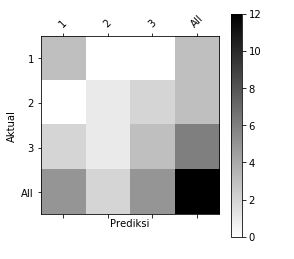
\includegraphics[width=1\textwidth]{figures/huda/chapter3/3.JPG}}
	\caption{Confusion Matrix}
	\label{h3}
\end{figure}
\item Voting pada random forest sebagaimana voting yaitu suara/hasil untuk setiap target yang diprediksi pada saat melakukan Random Forest. Pertimbangkan target prediksi dengan voting terbanyak/tertinggi sebagai prediksi akhir dari algoritma random forest. Contoh ilustrasi dapat dilihat pada gambar \ref{h4}.
\begin{figure}[!htbp]
	\centerline{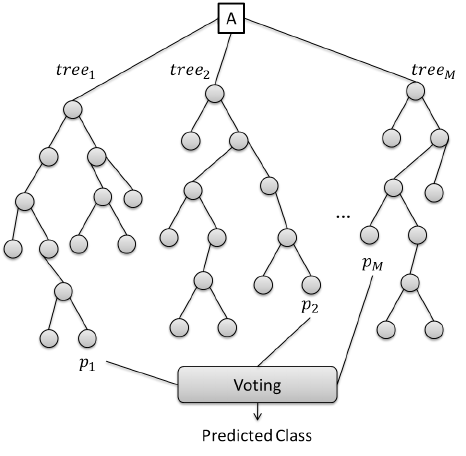
\includegraphics[width=1\textwidth]{figures/huda/chapter3/4.png}}
	\caption{Voting}
	\label{h4}
\end{figure}
\end{enumerate}

\subsection{Praktek Program}
\begin{enumerate}
\item 
\begin{verbatim}
import pandas as huda
a = huda.Series(['Ahmad', 'Syaf', 'Rizal', 'Huda', 'Mubarrok'],
index = [1, 2, 3, 4, 5])
print (a)
\end{verbatim}
\subitem Baris pertama pada codingan, yaitu import pandas as huda yang artinya kita akan mengimport librari pandas dari python dengan inisiasi huda.
\subitem Baris kedua pada codingan, yaitu Variabel a didefinisikan data data yang sudah dibuat seperti daftar nama dengan menggunakan huda.Series. Series adalah object satu dimensi yang serupa dengan kolom di dalam tabel.
\subitem Baris ketiga pada codingan, yaitu index digunakan untuk melabeli data dengan dimulai dari nomor 1...5, jika tidak label default akan dimulai dari 0,1,2...
\subitem Baris keempat pada codingan, yaitu digunakan untuk mencetak atau menampilkan data pada variabel a yang sudah dibuat sebelumnya.
\subitem Untuk hasilnya dapat dilihat pada gambar \ref{h5}.
\begin{figure}[!htbp]
	\centerline{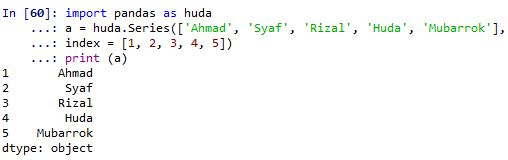
\includegraphics[width=1\textwidth]{figures/huda/chapter3_praktek/1.JPG}}
	\caption{Aplikasi Menggunakan Pandas}
	\label{h5}
\end{figure}
\item 
\begin{verbatim}
import numpy as huda
print (huda.arange(50, 101)) 
\end{verbatim}
\subitem Baris pertama pada codingan, yaitu import numpy as huda yang artinya kita akan mengimport librari numpy dari python dengan inisiasi huda.
\subitem Baris kedua pada codingan, yaitu digunakan untuk mencetak atau menampilkan data dengan menggunakan huda.arange untuk membuat array dengan bilangan sekuensial dari mulai nilai awal 50 sampai sebelum 101 dengan berurutan.
\subitem Untuk hasilnya dapat dilihat pada gambar \ref{h6}.
\begin{figure}[!htbp]
	\centerline{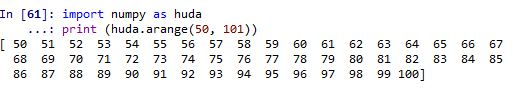
\includegraphics[width=1\textwidth]{figures/huda/chapter3_praktek/2.JPG}}
	\caption{Aplikasi Menggunakan Numpy}
	\label{h6}
\end{figure}
\item 
\begin{verbatim}
import matplotlib.pyplot as huda
huda.plot([0,1,3,5,7,8,10],[25, 35, 30, 45, 50, 45, 30])
huda.show()
\end{verbatim}
\subitem Baris pertama pada codingan, yaitu import matplotlib.pyplot as huda yang artinya kita akan mengimport librari matplotlib dengan class pyplot dari python dengan inisiasi huda.
\subitem Baris kedua pada codingan, yaitu digunakan untuk memasukkan data dengan insiai huda pada class plot dengan nilai x dan y yg sudah ditentukkan.
\subitem Baris ketiga pada codingan, yaitu digunakan untuk mencetak atau menampilkan data dengan inisiai huda.show nantinya keluaranyya berupa grafik.
\subitem Untuk hasilnya dapat dilihat pada gambar \ref{h7}.
\begin{figure}[!htbp]
	\centerline{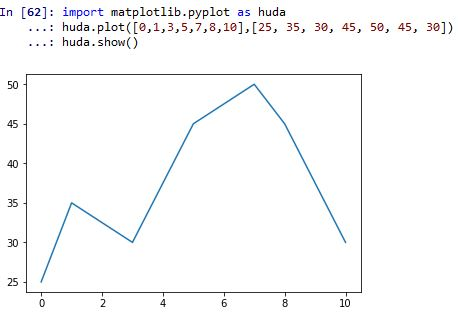
\includegraphics[width=1\textwidth]{figures/huda/chapter3_praktek/3.JPG}}
	\caption{Aplikasi Menggunakan Matplotlib}
	\label{h7}
\end{figure}
\item Menjalankan Klasifikasi Random Forest.
\subitem Pada gambar \ref{h8} berfungsi untuk membaca data yang berupa image\_attribute\_labels dengan format text file. Dengan mendefinisikan variabel imgatt yang berisikan value untuk membaca data, juga menggunakan code untuk skip data yang mengandung bad lines agar tidak terjadi eror pada saat pembacaan file.
\begin{figure}[!htbp]
	\centerline{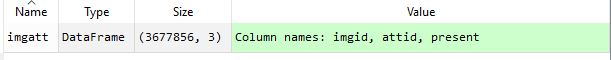
\includegraphics[width=1\textwidth]{figures/huda/chapter3_praktek/4.JPG}}
	\caption{Hasil 1 Random Forest}
	\label{h8}
\end{figure}
\subitem Pada gambar \ref{h9} yaitu mengembalikan baris n teratas (5 secara default) dari dataframe imgatt.
\begin{figure}[!htbp]
	\centerline{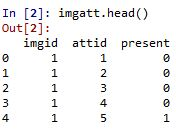
\includegraphics[width=1\textwidth]{figures/huda/chapter3_praktek/5.JPG}}
	\caption{Hasil 2 Random Forest}
	\label{h9}
\end{figure}
\subitem Pada gambar \ref{h10} yaitu menampilkan beberapa baris dan kolom dari dataframe imgatt.
\begin{figure}[!htbp]
	\centerline{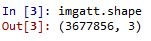
\includegraphics[width=1\textwidth]{figures/huda/chapter3_praktek/6.JPG}}
	\caption{Hasil 3 Random Forest}
	\label{h10}
\end{figure}
\subitem Pada gambar \ref{h11} yaitu variabel imgatt2 menggunakan function pivot untuk mengubah kolom jadi baris, dan baris jadi kolom dari dataframe sebelumnya.
\begin{figure}[!htbp]
	\centerline{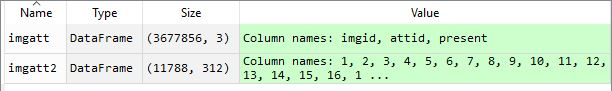
\includegraphics[width=1\textwidth]{figures/huda/chapter3_praktek/7.JPG}}
	\caption{Hasil 4 Random Forest}
	\label{h11}
\end{figure}
\subitem Pada gambar \ref{h12} yaitu imgatt2 head berfungsi untuk mengembalikan nilai teratas dari dataframe imgatt2.
\begin{figure}[!htbp]
	\centerline{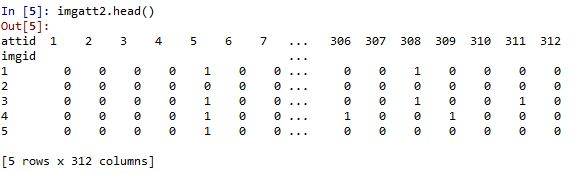
\includegraphics[width=1\textwidth]{figures/huda/chapter3_praktek/8.JPG}}
	\caption{Hasil 5 Random Forest}
	\label{h12}
\end{figure}
\subitem Pada gambar \ref{h13} yaitu menampilkan beberapa baris dan kolom dari dataframe imgatt2. 
\begin{figure}[!htbp]
	\centerline{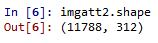
\includegraphics[width=1\textwidth]{figures/huda/chapter3_praktek/9.JPG}}
	\caption{Hasil 6 Random Forest}
	\label{h13}
\end{figure}
\subitem Pada gambar \ref{h14} yaitu melakukan pivot yang mana imgid menjadi index yang artinya unik.
\begin{figure}[!htbp]
	\centerline{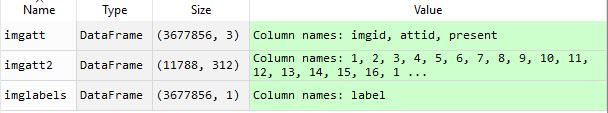
\includegraphics[width=1\textwidth]{figures/huda/chapter3_praktek/10.JPG}}
	\caption{Hasil 7 Random Forest}
	\label{h14}
\end{figure}
\subitem Pada gambar \ref{h15} yaitu memuat jawabannya yang berisi apakah burung itu termasuk dalam spesies yang mana. Dua kolomnya terdiri dari imgid dan label.
\begin{figure}[!htbp]
	\centerline{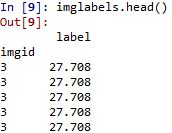
\includegraphics[width=1\textwidth]{figures/huda/chapter3_praktek/11.JPG}}
	\caption{Hasil 8 Random Forest}
	\label{h15}
\end{figure}
\subitem Pada gambar \ref{h16} yaitu menunjukkan 11788 baris dan 1 kolom. Dimana kolom itu adalah jenis spesies burungnya.
\begin{figure}[!htbp]
	\centerline{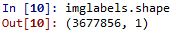
\includegraphics[width=1\textwidth]{figures/huda/chapter3_praktek/12.JPG}}
	\caption{Hasil 9 Random Forest}
	\label{h16}
\end{figure}
\subitem Pada gambar \ref{h17} yaitu join antara imgatt2 dengan imglabels dikarenakan isinya sama. Sehingga kita bisa mendapatkan data ciri dan data jawabannya/labelnya sehingga bisa dikategorikan supervised learning.
\begin{figure}[!htbp]
	\centerline{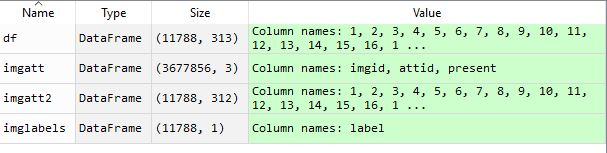
\includegraphics[width=1\textwidth]{figures/huda/chapter3_praktek/13.JPG}}
	\caption{Hasil 10 Random Forest}
	\label{h17}
\end{figure}
\subitem Pada gambar \ref{h18} yaitu menghilangkan label yang didepan, dan menggunakan label yang paling belakang yang baru di join.
\begin{figure}[!htbp]
	\centerline{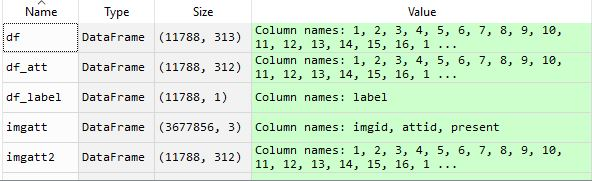
\includegraphics[width=1\textwidth]{figures/huda/chapter3_praktek/14.JPG}}
	\caption{Hasil 11 Random Forest}
	\label{h18}
\end{figure}
\subitem Pada gambar \ref{h19} yaitu mengecek 5 data teratas dari df att.
\begin{figure}[!htbp]
	\centerline{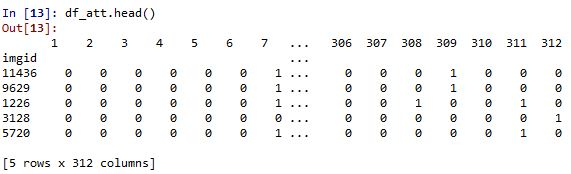
\includegraphics[width=1\textwidth]{figures/huda/chapter3_praktek/15.JPG}}
	\caption{Hasil 11 Random Forest}
	\label{h19}
\end{figure}
\subitem Pada gambar \ref{h20} yaitu mengecek 5 data teratas dari df label.
\begin{figure}[!htbp]
	\centerline{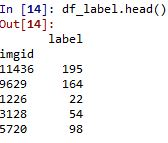
\includegraphics[width=1\textwidth]{figures/huda/chapter3_praktek/16.JPG}}
	\caption{Hasil 12 Random Forest}
	\label{h20}
\end{figure}
\subitem Pada gambar \ref{h21} yaitu 8000 row pertama sebagai data training sisanya sebagai data testing dengan membagi menjadi dua bagian.
\begin{figure}[!htbp]
	\centerline{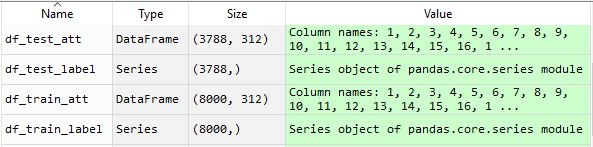
\includegraphics[width=1\textwidth]{figures/huda/chapter3_praktek/17.JPG}}
	\caption{Hasil 13 Random Forest}
	\label{h21}
\end{figure}
\subitem Pada gambar \ref{h22} yaitu memanggil kelas RandomForestClassifier. max features diartikan sebagai berapa banyak kolom pada setiap tree dengan isi maksimum 50.
\begin{figure}[!htbp]
	\centerline{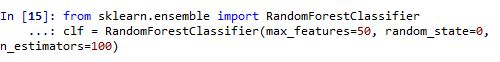
\includegraphics[width=1\textwidth]{figures/huda/chapter3_praktek/18.JPG}}
	\caption{Hasil 14 Random Forest}
	\label{h22}
\end{figure}
\subitem Pada gambar \ref{h23} yaitu melakukan fit untuk membangun random forest yang sudah ditentukan dengan maksimum fitur sebanya 50 untuk perpohonnya.
\begin{figure}[!htbp]
	\centerline{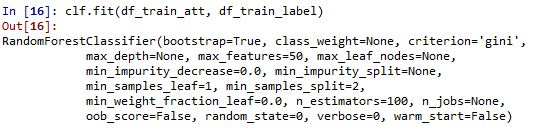
\includegraphics[width=1\textwidth]{figures/huda/chapter3_praktek/19.JPG}}
	\caption{Hasil 15 Random Forest}
	\label{h23}
\end{figure}
\subitem Pada gambar \ref{h24} yaitu menampilkan hasil prediksi dari random forest sebelumnya.
\begin{figure}[!htbp]
	\centerline{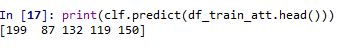
\includegraphics[width=1\textwidth]{figures/huda/chapter3_praktek/20.JPG}}
	\caption{Hasil 16 Random Forest}
	\label{h24}
\end{figure}
\subitem Pada gambar \ref{h25} yaitu menampilkan besaran akurasinya dari prediksi diatas atau score perolehan dari klasifikasi.
\begin{figure}[!htbp]
	\centerline{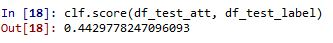
\includegraphics[width=1\textwidth]{figures/huda/chapter3_praktek/21.JPG}}
	\caption{Hasil 17 Random Forest}
	\label{h25}
\end{figure}
\item Menjalankan Confusion Matrix.
\subitem Pada gambar \ref{h26} yaitu menyatukan Random Forest ke dalam Confusion Matrix
\begin{figure}[!htbp]
	\centerline{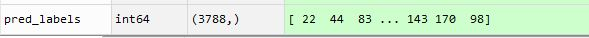
\includegraphics[width=1\textwidth]{figures/huda/chapter3_praktek/22.JPG}}
	\caption{Hasil 1 Confusion Matrix}
	\label{h26}
\end{figure}
\subitem Pada gambar \ref{h27} yaitu menampilkan hasil dari gambar sebekumnya dengan array pada perintah cm.
\begin{figure}[!htbp]
	\centerline{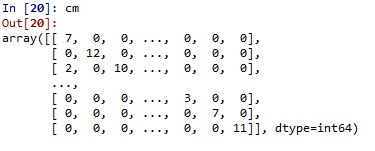
\includegraphics[width=1\textwidth]{figures/huda/chapter3_praktek/23.JPG}}
	\caption{Hasil 2 Confusion Matrix}
	\label{h27}
\end{figure}
\subitem Pada gambar \ref{h28} yaitu Plotting Confusion Matrix dengan librari Matplotlib.
\begin{figure}[!htbp]
	\centerline{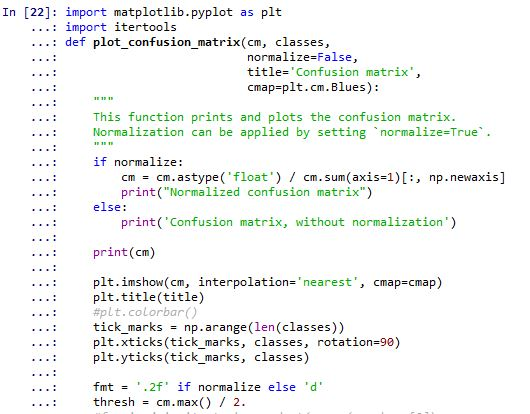
\includegraphics[width=1\textwidth]{figures/huda/chapter3_praktek/24.JPG}}
	\caption{Hasil 3 Confusion Matrix}
	\label{h28}
\end{figure}
\subitem Pada gambar \ref{h29} yaitu Set plot sumbunya sesuai dengan nama datanya dan membaca file classes.txt.
\begin{figure}[!htbp]
	\centerline{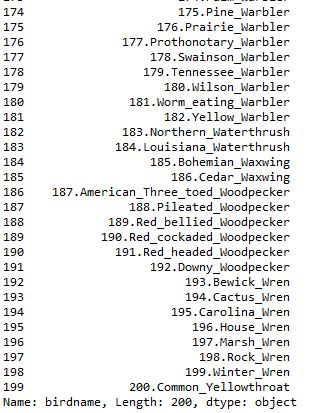
\includegraphics[width=1\textwidth]{figures/huda/chapter3_praktek/25.JPG}}
	\caption{Hasil 4 Confusion Matrix}
	\label{h29}
\end{figure}
\subitem Pada gambar \ref{h30} yaitu Plot hasil perubahan label yang sudah dilakukan.
\begin{figure}[!htbp]
	\centerline{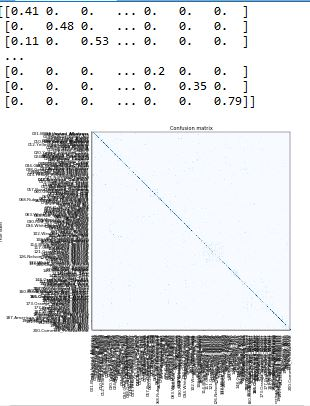
\includegraphics[width=1\textwidth]{figures/huda/chapter3_praktek/26.JPG}}
	\caption{Hasil 5 Confusion Matrix}
	\label{h30}
\end{figure}
\item Menjalankan Klasifikasi SVM dan Decision Tree.
\subitem Pada gambar \ref{h31} yaitu klasifikasi dengan decission tree dengan dataset yang sama dan akan muncul akurasi prediksinya.
\begin{figure}[!htbp]
	\centerline{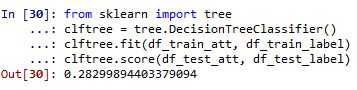
\includegraphics[width=1\textwidth]{figures/huda/chapter3_praktek/27.JPG}}
	\caption{Hasil 1 Klasifikasi SVM dan Decision Tree}
	\label{h31}
\end{figure}
\subitem Pada gambar \ref{h32} yaitu  klasifikasi dengan SVM dengan dataset yang sama dan akan muncul akurasi prediksinya.
\item Menjalankan Cross Validation.
\begin{figure}[!htbp]
	\centerline{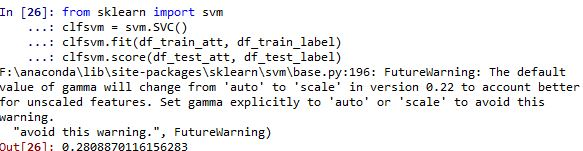
\includegraphics[width=1\textwidth]{figures/huda/chapter3_praktek/28.JPG}}
	\caption{Hasil 2 Klasifikasi SVM dan Decision Tree}
	\label{h32}
\end{figure}
\subitem Pada gambar \ref{h33} yaitu Cross Validation untuk  Random Forest.
\begin{figure}[!htbp]
	\centerline{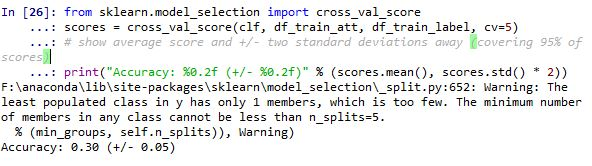
\includegraphics[width=1\textwidth]{figures/huda/chapter3_praktek/29.JPG}}
	\caption{Hasil 1 Cross Validation}
	\label{h33}
\end{figure}
\subitem Pada gambar \ref{h34} yaitu Cross Validation untuk Decission Tree.
\begin{figure}[!htbp]
	\centerline{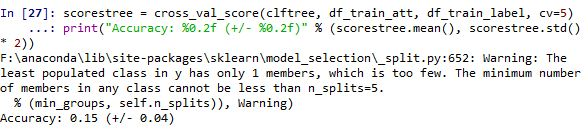
\includegraphics[width=1\textwidth]{figures/huda/chapter3_praktek/30.JPG}}
	\caption{Hasil 2 Cross Validation}
	\label{h34}
\end{figure}
\subitem Pada gambar \ref{h35} yaitu Cross Validation untuk SVM.
\begin{figure}[!htbp]
	\centerline{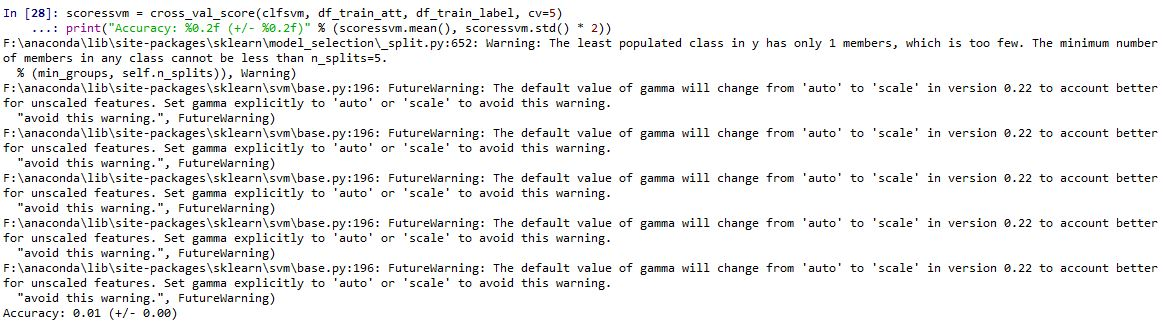
\includegraphics[width=1\textwidth]{figures/huda/chapter3_praktek/31.JPG}}
	\caption{Hasil 3 Cross Validation}
	\label{h35}
\end{figure}
\item Menjalankan Pengamatan Komponen Informasi.
\subitem Pada gambar \ref{h36} yaitu untuk mengetahui berapa banyak tree yang dibuat, berapa banyak atribut yang dipakai dan informasi lainnya.
\begin{figure}[!htbp]
	\centerline{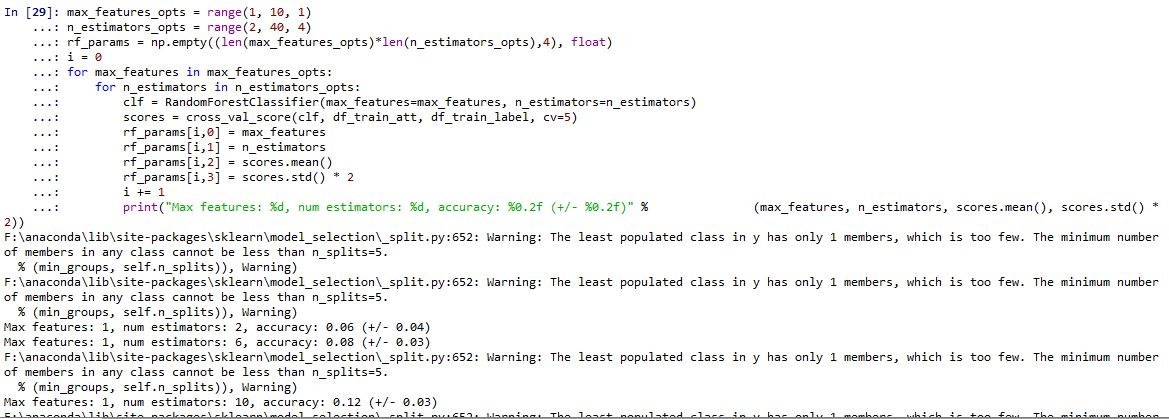
\includegraphics[width=1\textwidth]{figures/huda/chapter3_praktek/32.JPG}}
	\caption{Hasil 1 Pengamatan Komponen Informasi}
	\label{h36}
\end{figure}
\subitem Pada gambar \ref{h37} yaitu hasil dari plotting komponen informasi agar dapat dibaca.
\begin{figure}[!htbp]
	\centerline{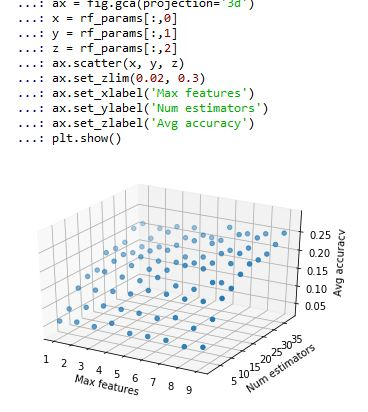
\includegraphics[width=1\textwidth]{figures/huda/chapter3_praktek/33.JPG}}
	\caption{Hasil 2 Pengamatan Komponen Informasi}
	\label{h37}
\end{figure}
\end{enumerate}

\subsection{Penanganan Eror}
\begin{enumerate}
\item Screenshootan eror ada pada gambar \ref{h38}.
\begin{figure}[!htbp]
	\centerline{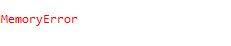
\includegraphics[width=1\textwidth]{figures/huda/chapter3_praktek/eror.JPG}}
	\caption{Eror}
	\label{h38}
\end{figure}
\item 
\begin{verbatim}
from sklearn.model_selection import cross_val_score
scores = cross_val_score(clf, df_train_att, df_train_label, cv=5)
print("Accuracy: %0.2f (+/- %0.2f)" % (scores.mean(), scores.std() * 2))
\end{verbatim}
\subitem 
\begin{verbatim}
scorestree = cross_val_score(clftree, df_train_att, df_train_label, cv=5)
print("Accuracy: %0.2f (+/- %0.2f)" % (scorestree.mean(), scorestree.std() * 2))
\end{verbatim}
\subitem 
\begin{verbatim}
scoressvm = cross_val_score(clfsvm, df_train_att, df_train_label, cv=5)
print("Accuracy: %0.2f (+/- %0.2f)" % (scoressvm.mean(), scoressvm.std() * 2))
\end{verbatim}
\subitem 
\begin{verbatim}
max_features_opts = range(1, 10, 1)
n_estimators_opts = range(2, 40, 4)
rf_params = np.empty((len(max_features_opts)*len(n_estimators_opts),4), float)
i = 0
for max_features in max_features_opts:
    for n_estimators in n_estimators_opts:
        clf = RandomForestClassifier(max_features=max_features, n_estimators=n_estimators)
        scores = cross_val_score(clf, df_train_att, df_train_label, cv=5)
        rf_params[i,0] = max_features
        rf_params[i,1] = n_estimators
        rf_params[i,2] = scores.mean()
        rf_params[i,3] = scores.std() * 2
        i += 1
        print("Max features: %d, num estimators: %d, accuracy: %0.2f (+/- %0.2f)" %
\end{verbatim}
\item Solusi pemecahan masalah tersebut yaitu dengan cara mengubah pada codingan dibawah in yang awalnya datanya 8000 menjadi 1000 semua dan max\_featurenya awalnya 50 menjadi 25.
\subitem 
\begin{verbatim}
df_train_att = df_att[:1000]
df_train_label = df_label[:1000]
df_test_att = df_att[1000:]
df_test_label = df_label[1000:]

df_train_label = df_train_label['label']
df_test_label = df_test_label['label']

from sklearn.ensemble import RandomForestClassifier
clf = RandomForestClassifier(max_features=25, random_state=0, n_estimators=100)
\end{verbatim}
\subitem Jika sudah dilakukan maka langkah selanjutnya yaitu kita tinggal merunning ulang dari awal hingga data tersebut berhasil diajalankan
\end{enumerate}